\chapter{Effective Field Theory}
\label{chap:EFT}

The concept of effective interactions has been around for nearly a century since Fermi first introduced it in 1933~\cite{Fermi:1933jpa} to explain the $\upbeta$ decay. The modern approach to effective interactions builds on the assumption that there is a separation between energy scales of different physics phenomena. When describing low-energy physics, the heavy mediators can be approximated to be point-like, and thus described by an effective coupling. This type of approach, collectively known as \ac{EFT}, has been very successful in simplifying calculations and describing low-energy experiments with stunning precisions. Depending on the energy scale at which \acp{EFT} are operating, they can be classified into different versions. One version of the \ac{EFT} that operates below the \ac{EW} scale and integrates out all the heavy fields is called the \ac{LEFT}, which is described in \autoref{sec:LEFT}. Another version of the \ac{EFT} that operators above the \ac{EW} scale is called the \ac{SMEFT}. It retains all the \ac{SM} fields and \sm~gauge symmetry. A description of the \ac{SMEFT} is given in \autoref{sec:SMEFT}.

\section{Low-Energy EFT}
\label{sec:LEFT}

It is safe to say that Fermi didn't have a complete description of the weak interactions in 1933. Instead, he constructed a phenological model to explain the $\upbeta$ decay. In his theory, he modified the \ac{QED} to include the following interaction vertex between four fermion fields:

\begin{equation}
-\frac{G_{\textsf{F}}}{\sqrt{2}}(\bar{\psi}_{\textsf{p}}\mathrm{\Gamma}\psi_{\textsf{n}})(\bar{\psi}_{\textsf{e}}\mathrm{\Gamma}\psi_{\nu})
\end{equation}

where $G_{\textsf{F}}$ is known as the Fermi constant, $\psi$ are Dirac fields that represent neutron, proton, electron, and electron neutrino. $\mathrm{\Gamma}$ is a 4$\times$4 matrix that encodes the Lorentz structure of the effective interaction. 

From the point view of the \ac{SM}, the $\upbeta$ decay is described by the charged-current interaction, whose amplitude in perturbative theory can be derived from the Lagrangian specified in Equation~\ref{eq:LCC}:

\begin{equation}
\label{eq:beta}
\frac{1}{8}(\bar{u}\mathrm{\Gamma}d)\frac{g^2}{q^2-m_{W}^2}(\bar{e}\mathrm{\Gamma}\nu),
\end{equation}

where $q$ and $m_W$ are the momentum and mass of the W propagator, respectively, and $g$ is the strength of the $SU(2)_{L}$ gauge interaction as mentioned in \autoref{sec:Gauge}.

Because $m_W\approx$ 80.4 GeV, is considered to be a lot higher than the energy scale associated with the $\uptau$ decay. The momentum of the W boson can be ignored and Equation~\ref{eq:beta} reduces to:

\begin{equation}
\label{eq:beta2}
-\frac{g^2}{8m_{W}^2}(\bar{u}\mathrm{\Gamma}d)(\bar{e}\mathrm{\Gamma}\nu),
\end{equation}

which is exactly the Fermi's theory with:

\begin{equation}
\frac{G_{\textsf{F}}}{\sqrt{2}}=\frac{g^2}{8m_{W}^2}.
\end{equation}

As illustrated in Figure~\ref{fig:FermiEFT}, Fermi's theory of weak interaction works very well at low energy. However, it ultimately breaks down when the momentum transfer is high enough. 

\begin{figure}[tbh!]
 \begin{center}
 \begin{tabular}{cc}
 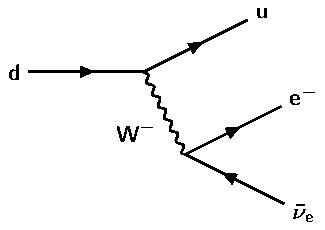
\includegraphics[width=0.45\textwidth]{figures/Part1/EFT/BetaDecay}&
 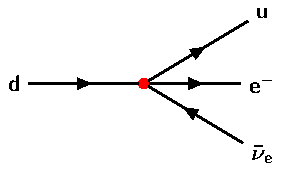
\includegraphics[width=0.45\textwidth]{figures/Part1/EFT/FermiTheory}\\
 \end{tabular}
 \caption{Representative Feynman diagrams for $\upbeta$ decay. The \ac{SM} description of this phenomenon with a massive weak mediator is illustrated on the left. At low energy, the heavy weak boson is approximated to be point-like in Fermi's theory of weak interactions, which is illustrated on the right. The effective coupling between four fermions indicated with a red dot, can be used to describe the same phenomenon.}
 \label{fig:FermiEFT}
 \end{center}
\end{figure}

The \ac{LEFT} that we know today is not that different from Fermi's original theory of weak interactions. It operates below the \ac{EW} scale, where the gauge symmetry of the \ac{SM} reduces to $SU(3)_{C}\bigotimes U(1)_{EM}$. It makes no explicit assumptions about the structure of the theory at higher energy. Except for the gauge bosons, the Higgs boson, and the top quark, all other fields are considered in the \ac{LEFT}. 

The \ac{LEFT} is usually deployed in a ``bottom-up'' way to model high-energy physics, whose structure is not yet known. For example, assuming new physics at a very high energy scale is responsible for the $\mathcal{R}(\textsf{D})$ anomaly described in \autoref{sec:BSM}, the phenomenon observed at low-energy experiments can be therefore parameterized by the \ac{LEFT}, as illustrated in Figure~\ref{fig:LEFT}.

\begin{figure}[tbh!]
 \begin{center}
 \begin{tabular}{cc}
 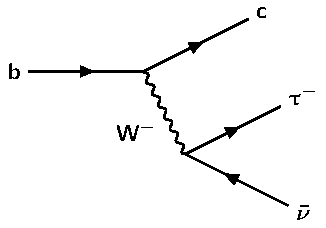
\includegraphics[width=0.45\textwidth]{figures/Part1/BSM/SMbtoc}&
 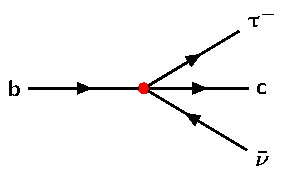
\includegraphics[width=0.5\textwidth]{figures/Part1/EFT/LEFT}
 \end{tabular}
 \caption{Representative Feynman diagram for b$\rightarrow$c transtion in the \ac{SM} (left). This process might also be enhanced by new physics with a much higher energy scale. The potential contributions from new physics can therefore be described by an effective coupling between four fermions, which is illustrated on the right.}
 \label{fig:LEFT}
 \end{center}
\end{figure}

\section{Standard Model EFT}
\label{sec:SMEFT}

The \ac{SM} can also be viewed as an \ac{EFT} as it is commonly accepted that it is not valid up to an arbitrarily high energy scale. This view leads to a different version of \ac{EFT}, known as the \ac{SMEFT}. The \ac{SMEFT} builds higher dimensional operators out of \ac{SM} fields to systematically study \ac{SM} deviations. These higher dimensional operators respect \sm~gauge symmetry and are added to \ac{SM} Lagrangian:

\begin{equation}
\label{eq:SMEFT}
\mathcal{L}_{\textsf{SMEFT}}=\mathcal{L}_{\textsf{SM}}^{(4)} + \frac{1}{\Lam}\WC{(5)}{}\OP{(5)}{}+ \frac{1}{\Lam^2}\sum_{a}\WC{(6)}{a}\OP{(6)}{a} + ...,
\end{equation}  

where $\mathcal{L}_{\text{SM}}^{(4)}$ is the renormalizable Lagrangian of the \ac{SM}. The $\OP{(n)}{}$ denote dimension-n nonrenormalizable operators, and $\WC{(n)}{}$ are the corresponding Wilson coefficients. The high dimensional operators are suppressed by powers of a mass scale $\Lambda$ where new physics is presumed to emerge. 

The only \ac{SM} gauge-invariant operator at dimension-five is the Weinberg operator~\cite{Weinberg:1979sa} of the following form

\begin{equation}
\OP{(5)}{}=(\phi\cdot\bar{L})(L\cdot\phi),
\end{equation}

where $\phi$ is the Higgs doublet mentioned in \autoref{sec:Higgs}. This operator gives rise to the Majorana mass terms for neutrinos upon \ac{EW} symmetry breaking:

\begin{equation}
m_{\textsf{Majorana}}=\WC{(5)}{}\frac{v^2}{\Lam},
\end{equation}

where $v$ is the vacuum expectation value mentioned in \autoref{sec:Higgs}.

Many more dimension-six operators are invariant under the \ac{SM} gauge transformations. They can be classified by the so-called Warsaw basis~\cite{Grzadkowski:2010es}. These operators are more relevant to this thesis as they can be formed by four fermionic fields that facilitate the flavor-violating $\ell\ell^{\prime}$qt interactions. A summary of these four-fermion operators is given in \autoref{sec:Signals}.